\section{Motivation}

As nuclear engineers, we are concerned with the behaviour of neutrons in nuclear reactors due to their influence on reaction rates, criticality, hot spots, burn-up, etc. The governing neutron transport equation that we are most frequently interested in is:
\begin{equation}\label{eq:NTE}
\begin{split}
    \mathbf{\Omega}\cdot\nabla\psi(\mathbf{r},E,\mathbf{\Omega}) + \Sigma_\mathrm{t}(\mathbf{r},E)\psi(\mathbf{r},E,\mathbf{\Omega}) = \frac{\chi(E)}{4\pi k_\mathrm{eff}}\int^{\infty}_0\mathrm{d}E' \bar{\nu}\Sigma_\mathrm{f}(\mathbf{r},E')\phi(\mathbf{r},E') \\
    + \int^{\infty}_0\mathrm{d}E'\int_{4\pi}\mathrm{d}\Omega'\Sigma_\mathrm{s}(\mathbf{r},E'\rightarrow E, \mathbf{\Omega}'\rightarrow\mathbf{\Omega})\psi(\mathbf{r},E',\mathbf{\Omega}')\;\mathrm{,}
\end{split}
\end{equation}
where $\psi$ is the neutron angular flux which depends upon position, $\mathbf{r}$, neutron energy, $E$, and neutron direction, $\mathbf{\Omega}$, $\Sigma_x$ is a cross section (total, fission, and scattering), $\chi$ is the fission neutron energy spectrum, $k_\mathrm{eff}$ is the criticality eigenvalue, $\bar{\nu}$ is the average neutron production from fission, $\phi$ is the scalar neutron flux, and $\Sigma_s(\mathbf{r},E'\rightarrow E, \mathbf{\Omega}'\rightarrow \mathbf{\Omega})$ is the double-differential scattering cross section. However, no nuclear engineer solves this equation: either we use Monte Carlo where this equation is irrelevant or we solve an approximation of this equation.

The most ubiquitous approximation is the multigroup approximation, i.e., discretisation of the energy variable. We do this by asserting that in a given energy range (or energy group, $g$) the cross sections and flux are piecewise constant: $\Sigma_{x,g}$, $\psi_g$. We then define our multigroup flux as the integral of the continuous energy flux over the energy range $E\in [E_{g},E_{g-1}]$:
\begin{equation*}
    \psi_g(\mathbf{r},\mathbf{\Omega}) = \int^{E_{g-1}}_{E_g}\mathrm{d}E \psi(\mathbf{r},E,\mathbf{\Omega})\;\mathrm{,}
\end{equation*}
\begin{equation*}
    \phi_g(\mathbf{r}) = \int^{E_{g-1}}_{E_g}\mathrm{d}E \phi(\mathbf{r},E)\;\mathrm{.}
\end{equation*}
Integrating Eq.~\eqref{eq:NTE} over each energy group produces a set of equations of the form:
\begin{equation}\label{eq:NTE_MG}
\begin{split}
    \mathbf{\Omega}\cdot\nabla\psi_g(\mathbf{r},\mathbf{\Omega}) + \Sigma_{\mathrm{t},g}(\mathbf{r})\psi_g(\mathbf{r},\mathbf{\Omega}) = \frac{\chi_g}{4\pi k_\mathrm{eff}}\sum_{g'} \bar{\nu}\Sigma_{\mathrm{f},g'}(\mathbf{r})\phi_{g'}(\mathbf{r}) \\
    + \sum_{g'}\int_{4\pi}\mathrm{d}\Omega'\Sigma_{\mathrm{s},g'\rightarrow g}(\mathbf{r}, \mathbf{\Omega}'\rightarrow\mathbf{\Omega})\psi_{g'}(\mathbf{r},\mathbf{\Omega}')\;\mathrm{.}
\end{split}
\end{equation}
While this equation is an approximation of Eq.~\eqref{eq:NTE}, it can be valuable provided it preserves the reaction rates that would be obtained by solving Eq.~\eqref{eq:NTE}. More precisely, we want to ensure:
\begin{equation}
    \Sigma_{x,g}\phi_g = \int^{E_{g-1}}_{E_g}\mathrm{d}E\; \Sigma_x(E)\phi(E)\;\mathrm{.}
\end{equation}
This requirement in turn tells us exactly how to choose the values of $\Sigma_{x,g}$:
\begin{equation}\label{eq:MG}
    \Sigma_{x,g}=\frac{\int^{E_{g-1}}_{E_g}\mathrm{d}E\; \Sigma_x(E)\phi(E)}{\phi_g} = \frac{\int^{E_{g-1}}_{E_g}\mathrm{d}E\; \Sigma_x(E)\phi(E)}{\int^{E_{g-1}}_{E_g}\mathrm{d}E\; \phi(E)}\;\mathrm{.}
\end{equation}
In other words, $\Sigma_{x,g}$ should be a flux-weighted average of $\Sigma_x(E)$. This brings us to one of the central problems of nuclear engineering...

\begin{displayquote}
\textbf{``Wait a minute,'' you ask, ``the purpose of solving the transport equation is to get the flux, but I have to know the flux to compute the multi-group constants!''}

\textbf{-- The NJOY manual}
\end{displayquote}

Life could be worse, however: when neutrons are thermal, the spectrum is essentially Maxwellian. Meanwhile, when neutrons are fast, the fission spectrum is a good approximation and geometry effects are negligible -- in LWRs, neutrons do not spend significant time in the fast region anyway. In these two regions, we can (with some approximations or slightly finer energy discretisation) reasonably accurately evaluate cross sections using Eq.~\eqref{eq:MG}. In between, however, we do not have this luxury.

In this intermediate range, \textbf{cross sections are resonant} and sufficiently large such that \textbf{geometry effects} become important. Both of these means that the flux spectrum can be perturbed quite dramatically depending on the particular composition and configuration of a reactor. This is strongly related to the concept of spatial and energy self-shielding. We must somehow account for these resonance and geometry effects.

Despite this, we still manage to have a reasonably low number of energy groups while maintaining good accuracy in LWR calculations. This is illustrated with the WIM69 group structure in Fig.~\ref{fig:WIMS}.

\begin{figure}[h]
  \centering
  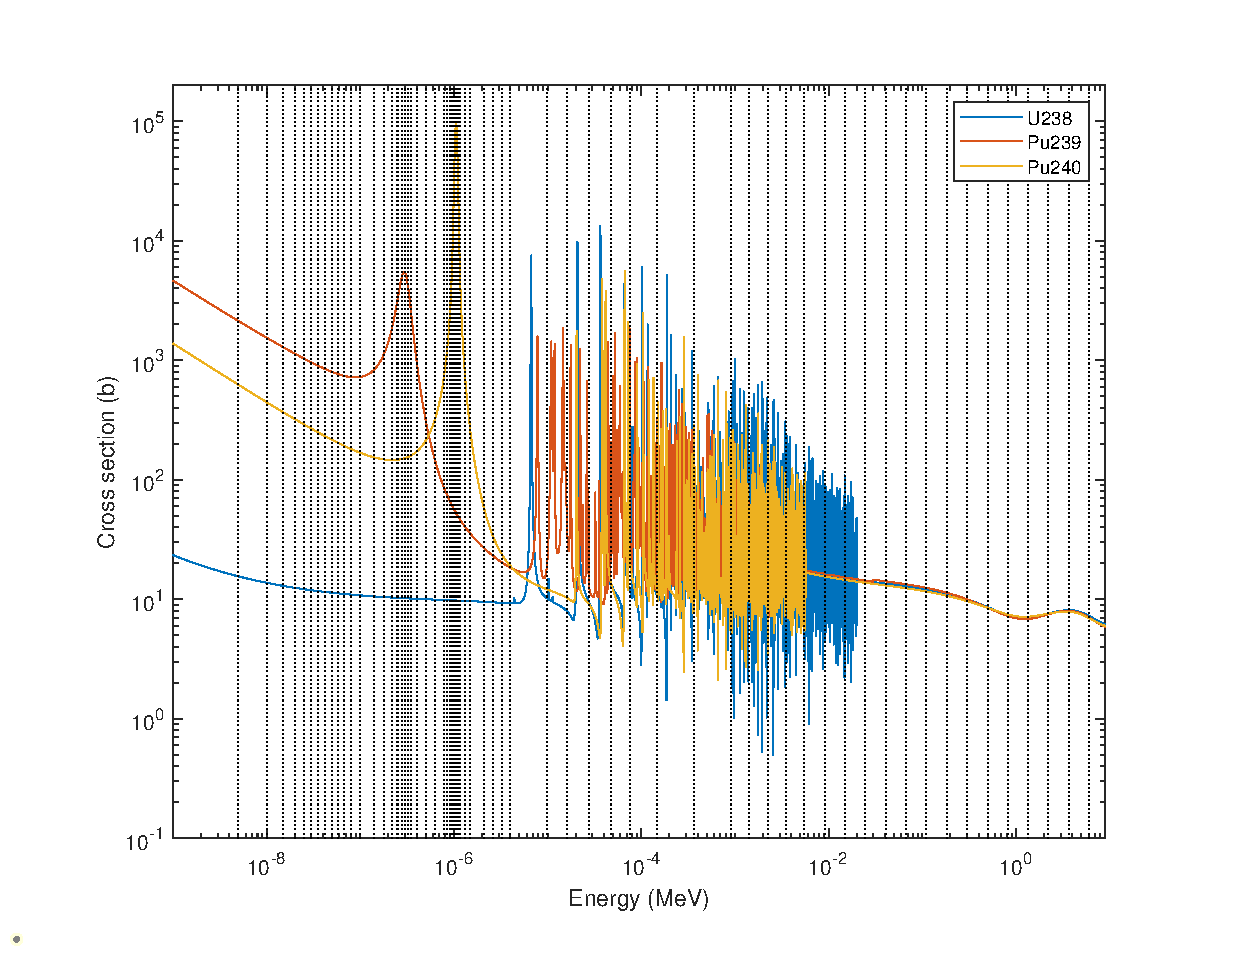
\includegraphics[scale=0.70]{./Figures/intro/cross_sections_WIMS69.eps} 
  \caption{WIMS69 group structure overlaid with some prominent nuclides.} 
  \label{fig:WIMS}
\end{figure}

This lecture series aims to partially explain how we can generate multigroup cross sections by coming up with sufficiently good approximations to the flux spectrum in a surprisingly wide number of conditions. The basic principles have been well known for a while, but are not often taught as they sit at the back of proprietary lattice physics code. Most of the content of this lecture series is ultimately about explaining the theoretical basis of the HEAD module in WIMS, for example. While there are several quite simple and important results that allow these codes to produce cross sections which are sufficiently accurate for reactor design, reaching these results is non-trivial. Perhaps the main purpose of this series is to convey that, as Eugene would often say, \textbf{``cross sections do not fall from the sky''}.

I should emphasise that the focus is tailored towards thermal reactors; the approximations that feature here were historically deemed acceptably accurate for thermal systems without exceeding the contemporary computational budget -- treatments for fast reactors tend to differ significantly. However, it remains an open question how relevant some of these methods will be in the future: many of the treatments described here could be and have been replaced by higher fidelity methods. Several lattice physics codes now employ fine-group slowing down equation solutions, while Monte Carlo is regularly used to generate cross sections for whole-core transport or diffusion simulations. History suggests that computation only becomes cheaper and the cost of conservatism becomes greater, so it will be interesting to see whether the methods discussed will persist for much longer.
